\documentclass[crop,tikz,]{standalone}

\begin{document}
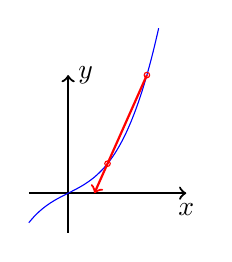
\begin{tikzpicture}
		 \draw[->,thick] (-0.5,0) -- (1.5,0) node[below] {$x$}; \draw[->,thick] (0,-0.5) -- (0,1.5) node[right] {$y$};
		 \draw[domain=-0.5:1.15, smooth, variable=\x, blue] plot ({\x}, {\x*\x*\x + \x/2});
		 \draw[red] (0.5,0.5^3+0.25) circle (1pt); \draw[red] (1,1.5) circle (1pt);
		 \draw[thick,red] (0.5,0.375) -- (1,1.5);
		 \draw[->,thick,red] (0.5,0.5^3+0.25) -- (0.5 - 0.1667,0);
\end{tikzpicture}
\end{document}